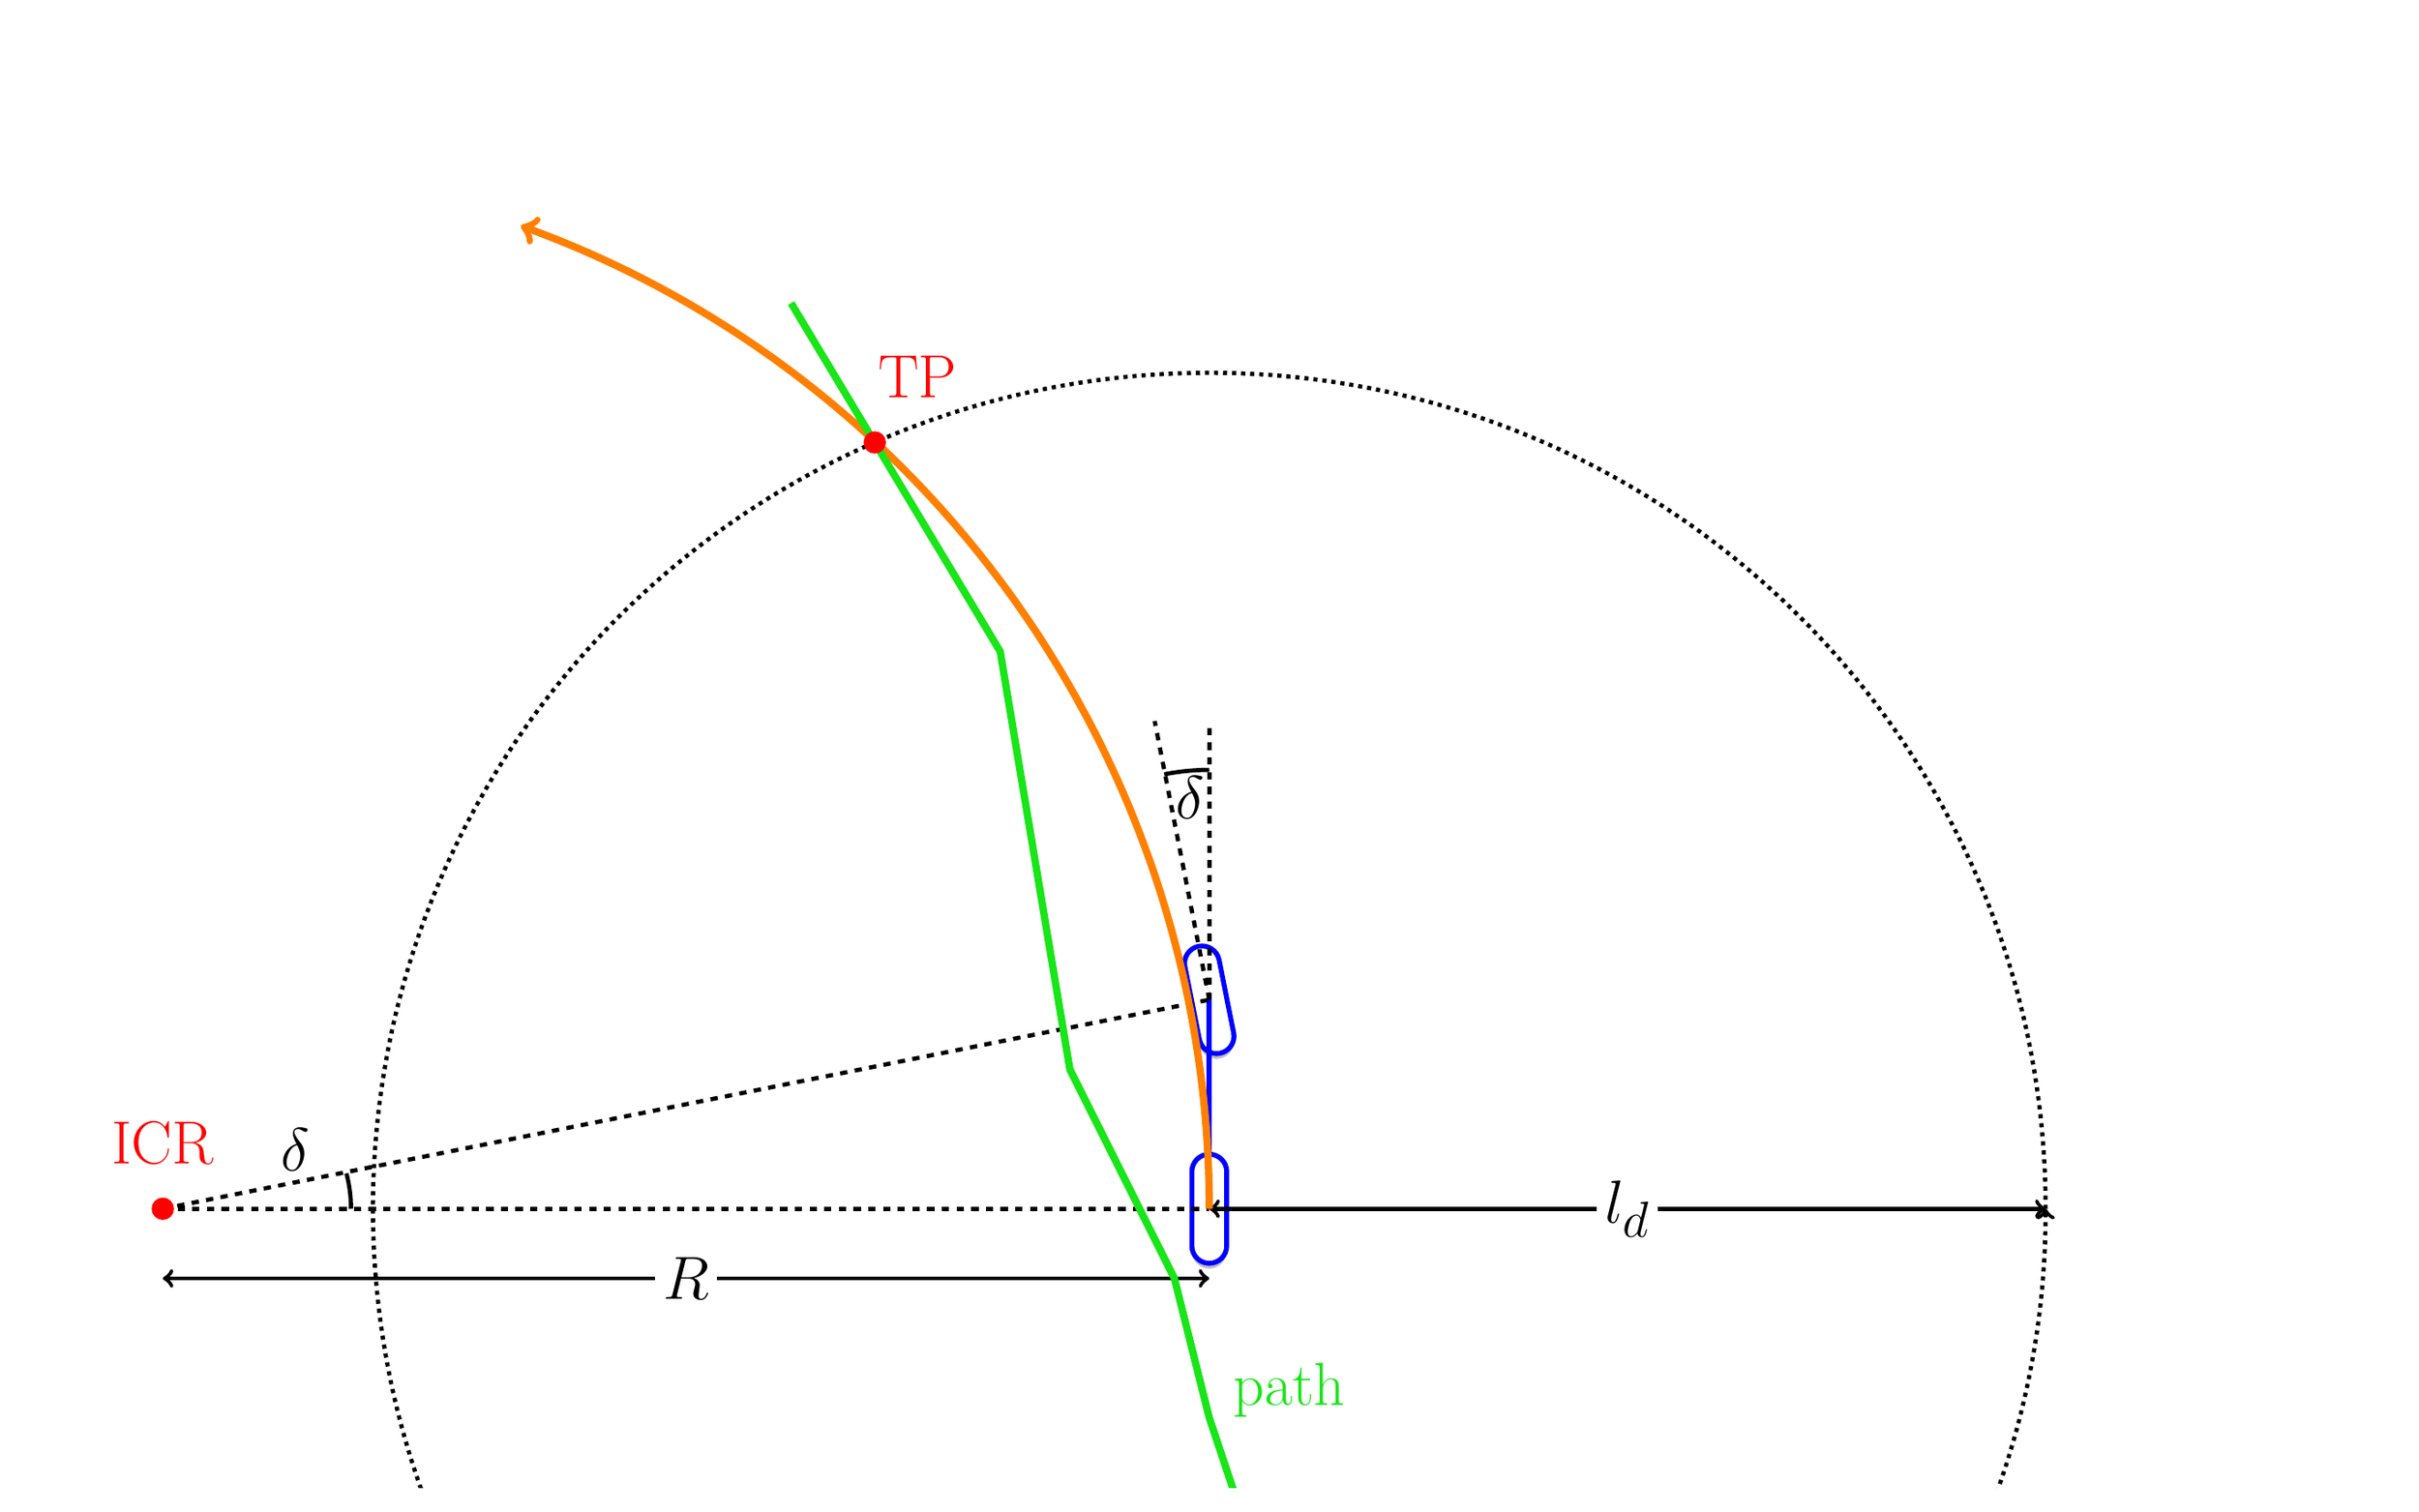
\begin{tikzpicture}[line width=1.7pt]
\usetikzlibrary{shapes.misc,shadows}
\usetikzlibrary{calc}
\usetikzlibrary{positioning,backgrounds}

\pgfmathsetmacro{\dist}{3}
\pgfmathsetmacro{\deltavar}{11.3}
\pgfmathsetmacro{\ax}{tan(90-\deltavar)*\dist*(-1)}
\pgfmathsetmacro{\lookahead}{12}
\pgfmathsetmacro{\cs}{17}
\pgfmathsetmacro{\csb}{4}


\path[clip] (-\cs,-\csb)--(-\cs,\cs)--(\cs,\cs)--(\cs, -\csb) --cycle;

% NODES
\node(tire1)[draw=blue, thick, fill=white, 
			shape=rounded rectangle,  
			drop shadow={opacity=.5,shadow xshift=0pt},
			minimum width=1.8cm, 
			minimum height=0.5cm,
			line width =2,
			rotate=90]  at (0,0)   {};
			
\node(tire2)[draw=blue, thick, fill=white, 
			shape=rounded rectangle,  
			drop shadow={opacity=.5,shadow xshift=0pt},
			minimum width=1.8cm, 
			minimum height=0.5cm,
			line width =2,
			rotate=\deltavar-90]  at (0,\dist)   {};
			
\node(triangle_left) at (\ax,0){};



% TRIANGLE
 \draw[line width=2, color=blue]  (tire1.center) -- (tire2.center); 
\draw[dashed]  (triangle_left.center) -- (tire2.center);
\draw[dashed]  (triangle_left.center) -- (tire1.center);

% length R and L 
\draw[<->]  (\ax, -1) -- (0,-1) node[midway, fill=white] {\Huge $R$};
%\draw[<->]  (1, 0) -- (1,\dist) node[midway, fill=white] {\Huge $L$};
\draw[<->]  (\lookahead, 0) -- (0,0) node[midway, fill=white] {\Huge $l_d$};

% angle delta top
\draw[dashed] (0, \dist) -- (0,\dist+4);
\draw[dashed] (0, \dist) -- ({-sin(\deltavar)*4},{\dist+4)});
\draw[color=black] (0,\dist+3.3) arc (90:90+\deltavar:3.3);
\draw (-0.27, \dist+2.9) node[black] {\Huge $\delta$};

 %angle delta left
\draw[color=black] ({\ax+2.7},0) arc (0:1.3*\deltavar:2);
\draw (\ax+1.9, 0.85) node[black] {\Huge $\delta$};
 
% circle 
 \draw[ ->, orange, line width=3] (0,0) arc (0:70:-\ax); 

% circle LookAhead
 \draw[ ->, dotted] (\lookahead,0) arc (0:360:\lookahead); 

% ICR
\node[red] at (\ax,0.5)[above]{\Huge ICR};
\draw[red, fill] (triangle_left) circle(0.13);

% PATH
\draw[green!80!gray, line width =3](1, -6) --(0,-3) -- (-0.5, -1) -- (-1,0) -- (-1.5,1) -- (-2,2) -- (-3, 8) -- (-6,13)  ;
\node[green!80!gray] at (0.6,-2.6)[right=-0.4]{\Huge path};

% target
\node[red] at (-4.8,11)[above right=0.5 and -0.1]{\Huge TP};
\draw[red, fill] (-4.8,11) circle(0.13);

\end{tikzpicture}